\chapter{System model}

\section{Scenarios}

\subsection{Passenger sign up, real time request, taxi movement}
Bob wants to go to the theater. He downloads the \mts{} app on his smartphone, he opens it and he finds the passenger sign up page. He inserts his name and surname, his address, and his personal citizen ID. After receiving confirmation of a successful operation, he logs in by tapping on the corresponding button. He finds three options: \emph{call a taxi now}, \emph{reserve a taxi for later}, \emph{view reservation history}. He decides to tap the \emph{call a taxi now} function. He finds a form where he inserts the destination address and the number of passengers. The system notifies him to turn his GPS on if he wants to call a taxi to his current location, otherwise he can manually insert a starting address. He taps \emph{confirm} and the system answers by confirming back and sending him the estimated waiting time.

Charlie is a taxi driver already logged in the system, who has given his availability by tapping on the \emph{driver available} button on his personal page in the app. He receives notification that he has been assigned to picking up Bob. He accepts by tapping on the big red \emph{accept} button on his screen, he revs up and goes to the given starting address.

After arriving at destination, Charlie sends Bob on his way and notifies the system that he is available again. The system tells him in which zone of the city he will have to move to keep general widespread taxi coverage.

\subsection{New reservation,  previous reservation modification}
Tom wants to go to the airport at 4.30 AM. Since he is a very anxious person, one week in advance he logs in to \mts{}, chooses the reservation function from his personal page and reserves a ride for the right day and time and destination and starting address. He is relieved in seeing that the system has confirmed his reservation.
Three days later, his anxiety growing, he thinks he should change the reservation in order to be at the airport one hour before what he had planned. He logs again in \mts{} and he chooses the \emph{reservation history} function: the system shows him all of his previous reservations, which in this case is just the one he had made three days earlier. He taps the reservation entry and it pops out the option to \emph{modify} or \emph{delete} it. He carefully taps on \emph{modify} (heavens forbid he deletes it) and he is prompted to insert again all necessary information. He sighs in relief when the system confirms again that everything went well.
Unfortunately, two hours before the scheduled arrival of his taxi (Tom is well awake, least he forgets something for the journey), the system sends him notification that his request cannot be fulfilled due to unexpected events arising outside the sphere of influence of the taxi company. Tom is somewhat taken aback, but, after all, he expected nothing less.

\subsection{Driver sign up and availability, assignment rejection, taxi queque handling}
Eve is a taxi driver. She downloads the \mts{} app and signs up as a taxi driver as per company policy. She is prompted to insert her name and surname, her address, her personal citizen ID, her license number and her car's plate number. The system checks that she is indeed a real, active taxi driver and that she is on the company payroll. After receiving confirmation of a successful operation, she logs in by tapping on the corresponding button.

After going to work one morning, she logs and signals her availability by tapping on the corresponding button on her personal page. Since it's the first time in the day, the app firstly interfaces with her car's GPS tracker, and goes then in waiting mode. After a while, her app comes to life and notifies her that she has ten minutes to pick up a passenger at a certain place. She is busy having a fat cream \emph{bombolone} for breakfast, so she declines.

The system receives Eve's reject and moves her at the end of her queue. At the same time, it notifies the next-in-line.

%%%%%%%%%%%%%%%%%%%%%%%%%%%%%%%%%%%%%%%%%
%%%%%%%%%%%%%%%%%%%%%%%%%%%%%%%%%%%%%%%%%

\section{Use cases and UML diagrams}
The following section gathers a collection of use cases and useful UML diagrams to better model the system in terms of main functionalities, flow of events, components, actors, and events.

\begin{figure}
\centering
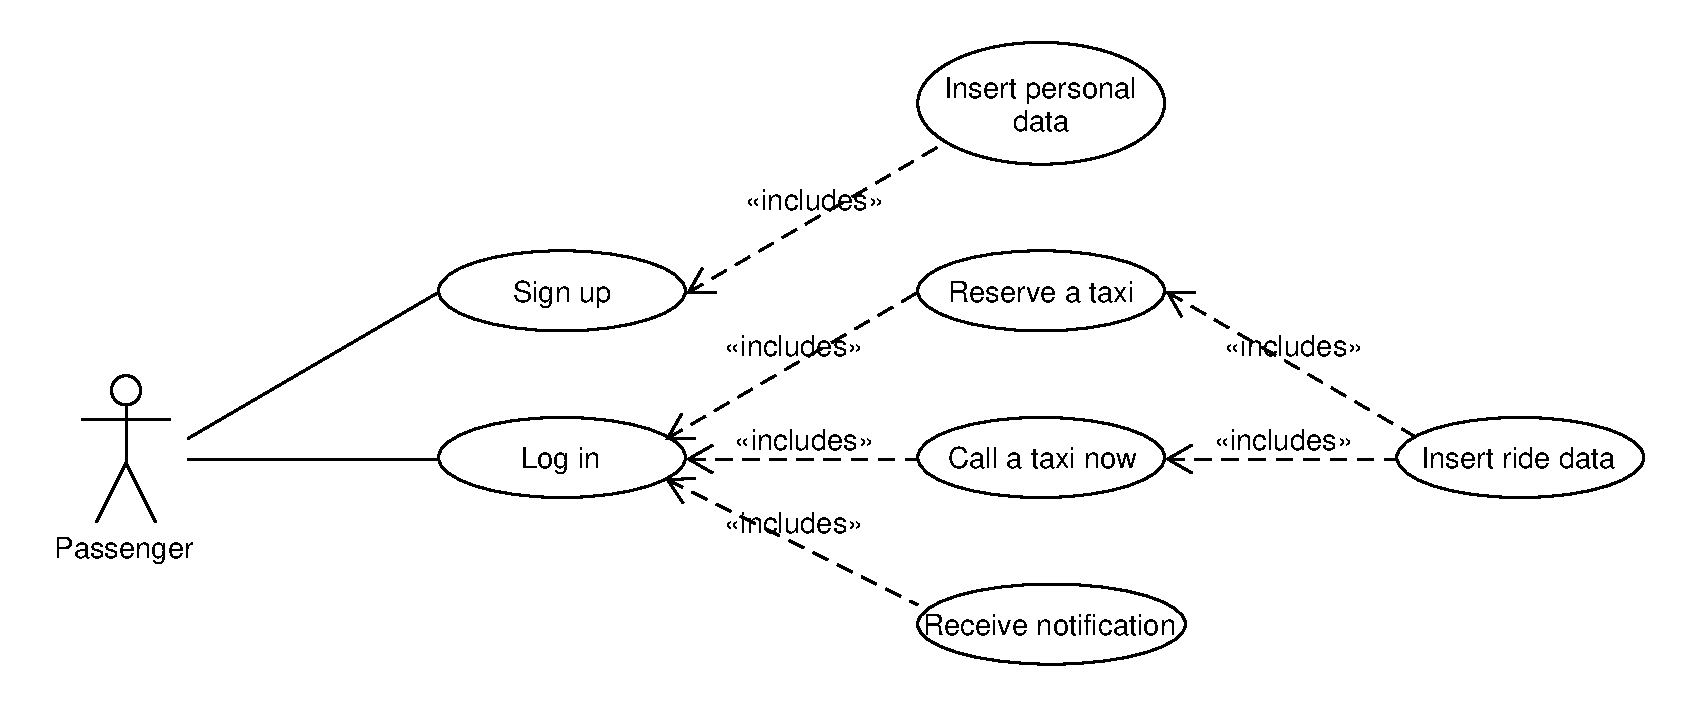
\includegraphics[width=\textwidth]{tex-images/usecase-passenger}
\caption{Overview of passenger use cases}
\end{figure}

\begin{figure}
\centering
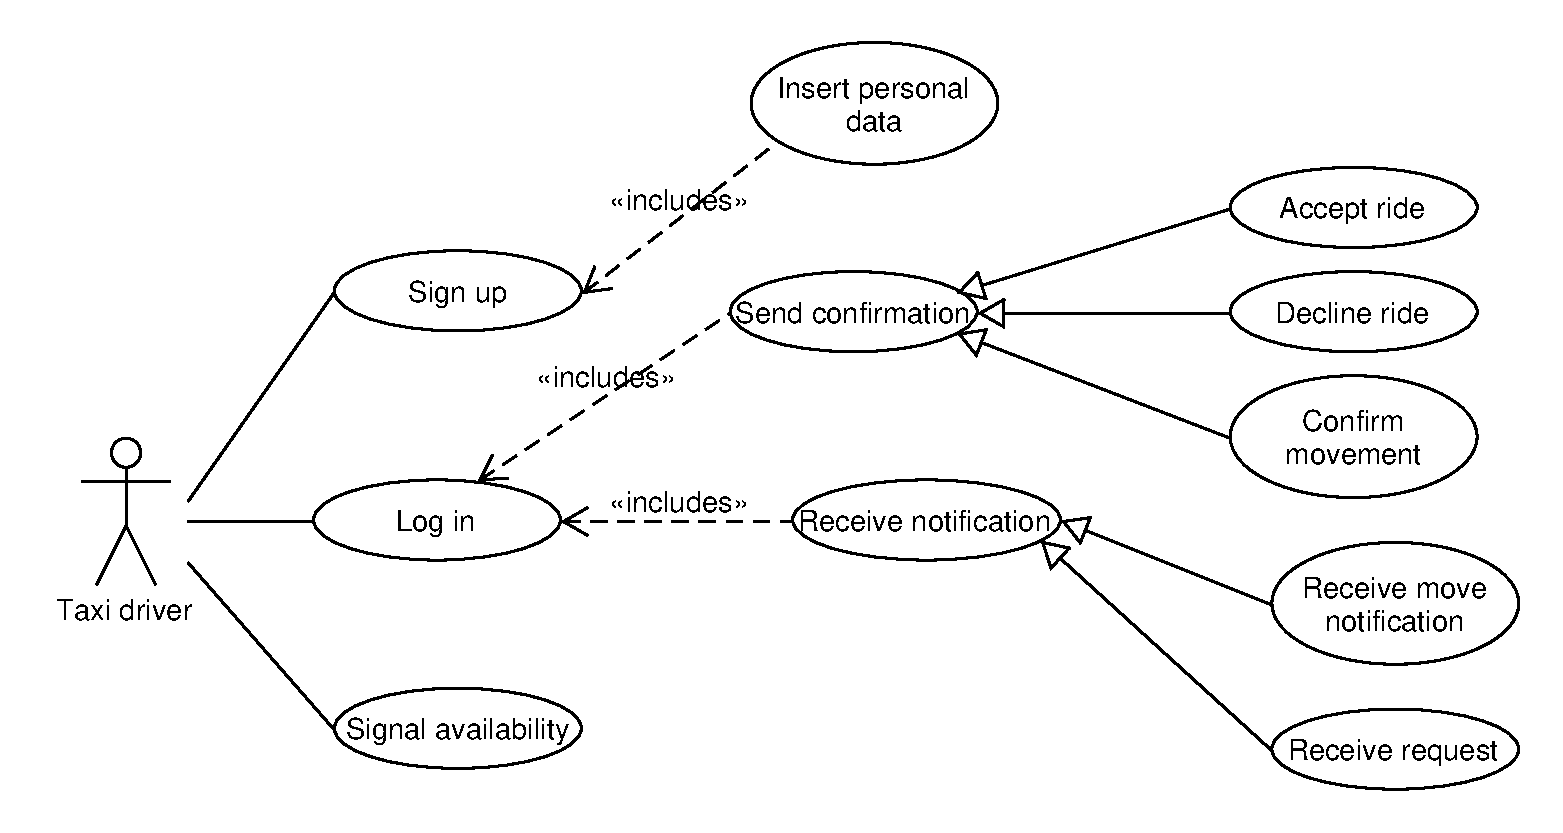
\includegraphics[width=\textwidth]{tex-images/usecase-driver}
\caption{Overview of taxi driver use cases}
\end{figure}


\begin{table}
\begin{center}
\begin{tabular}{lp{0.8\textwidth}}
\toprule
\textbf{Name}		&	\begin{itemize}
					\item Sign Up
					\end{itemize}	\\
\textbf{Actors}		&	\begin{itemize}
					\item Guest
					\end{itemize}	\\
\textbf{Entry conditions}	&	\begin{itemize}
					\item The guest isn't registered;
					\item The guest has opened the mobile app or the web site home page.
					\end{itemize}	\\
\textbf{Flow of events}	&	\begin{itemize}
					\item	The guest clicks on the \emph{Sign Up} button;
					\item	The system shows him the form to be filled;
					\item	The guest adds all requested information;
					\item	The guest clicks on the \emph{Confirm} button;
					\item	The system verifies the information, confirms the registration and stores new user's information.
					\end{itemize}	\\
\textbf{Exit conditions}	&	\begin{itemize}
					\item	The guest is correctly registered.
					\end{itemize}	\\
\textbf{Exceptions}	&	\begin{itemize}
					\item If the guest is already registered, the system notifies the user with a pop-up message;
					\item	If guest information are incomplete or incorrect, the system notifies the guest and asks him to rewrite them.
					\end{itemize}	\\
\bottomrule
\end{tabular}
\caption{Sign up use case}
\end{center}
\end{table}

\begin{figure}
\centering
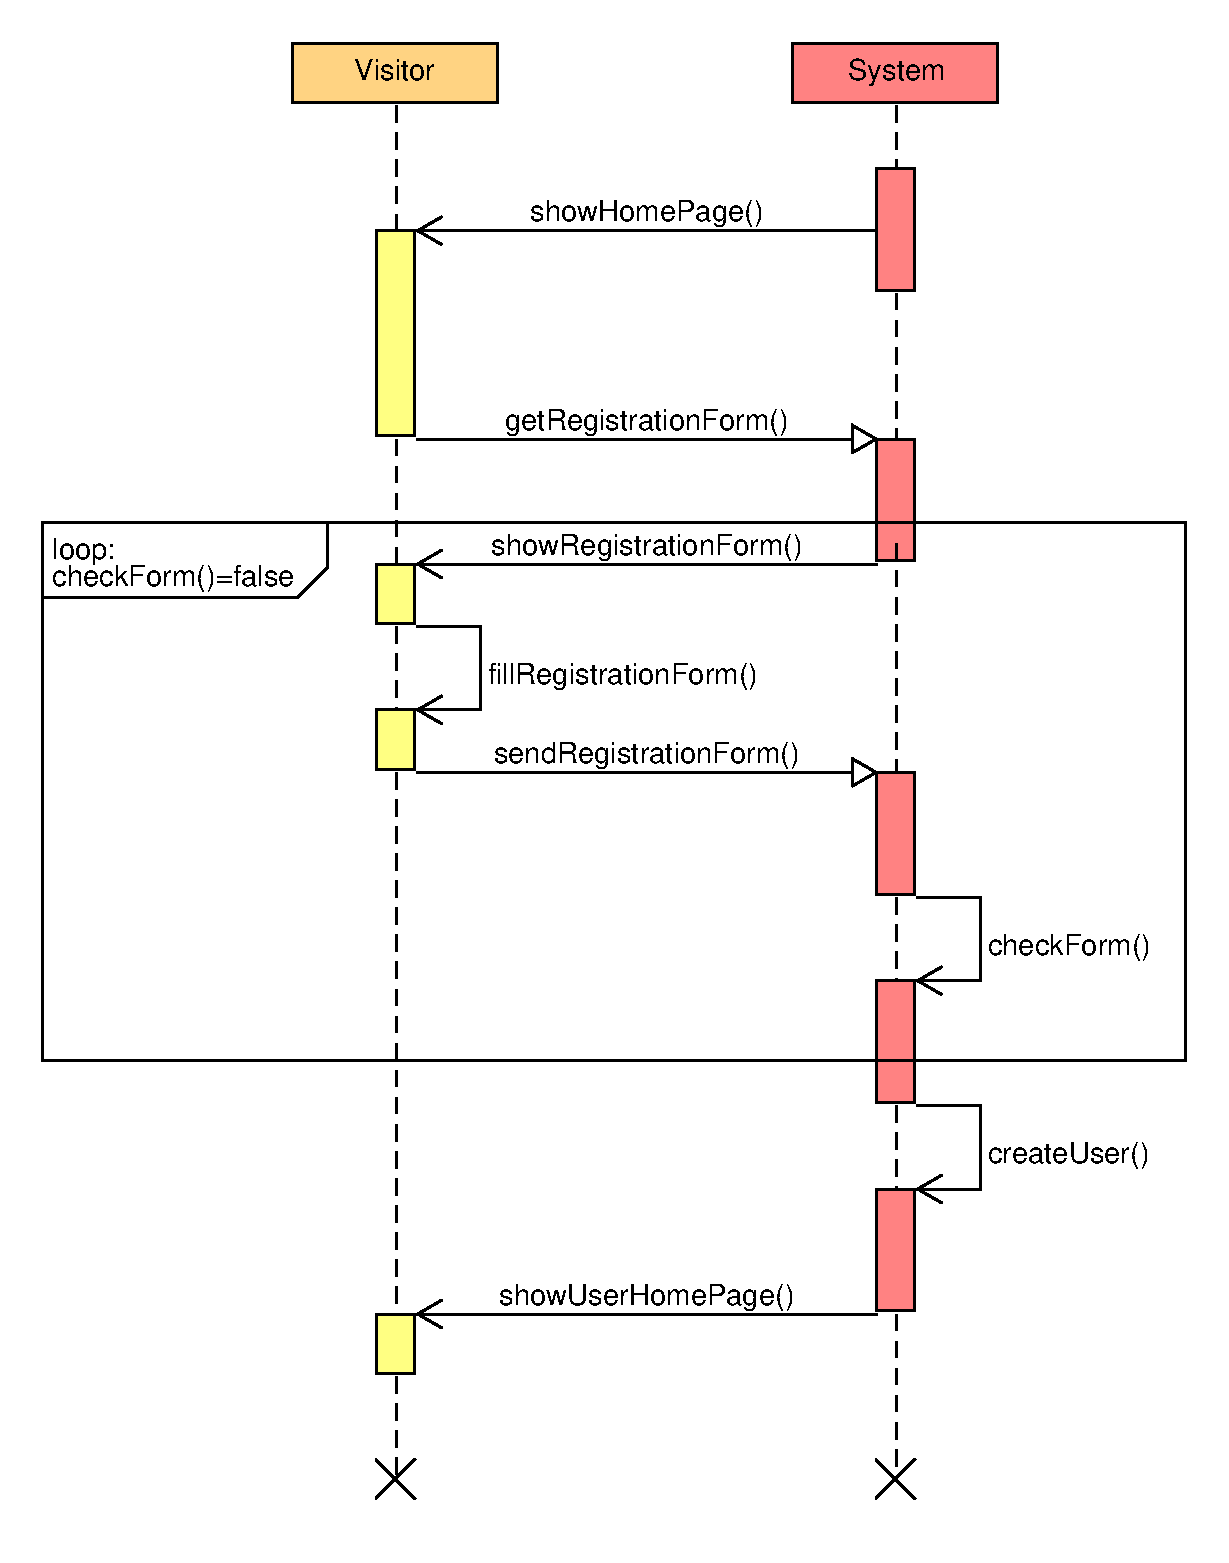
\includegraphics[width=\textwidth]{tex-images/sequence-signup}
\caption{Sign up sequence diagram}
\end{figure}



\begin{table}
\begin{center}
\begin{tabular}{lp{0.8\textwidth}}
\toprule
\textbf{Name}		&	\begin{itemize}
					\item Log In
					\end{itemize}	\\
\textbf{Actors}		&	\begin{itemize}
					\item Guest
					\end{itemize}	\\
\textbf{Entry conditions}	&	\begin{itemize}
					\item The guest is registered;
					\item	The guest has opened the mobile app or the web site home page.
					\end{itemize}	\\
\textbf{Flow of events}	&	\begin{itemize}
					\item	The guest clicks on the \emph{Log in} button;
					\item	The system shows him the form to be filled;
					\item	The guest writes user name and password:
					\item	The guest clicks on the \emph{Confirm} button;
					\item	The system verifies the information and shows user's home page.
					\end{itemize}	\\
\textbf{Exit conditions}	&	\begin{itemize}
					\item	The user is correctly logged in.
					\end{itemize}	\\
\textbf{Exceptions}	&	\begin{itemize}
					\item If validation process doesn't terminate well, the system ask the user to rewrite username and password.
					\end{itemize}	\\
\bottomrule
\end{tabular}
\caption{Log in use case}
\end{center}
\end{table}

\begin{figure}
\centering
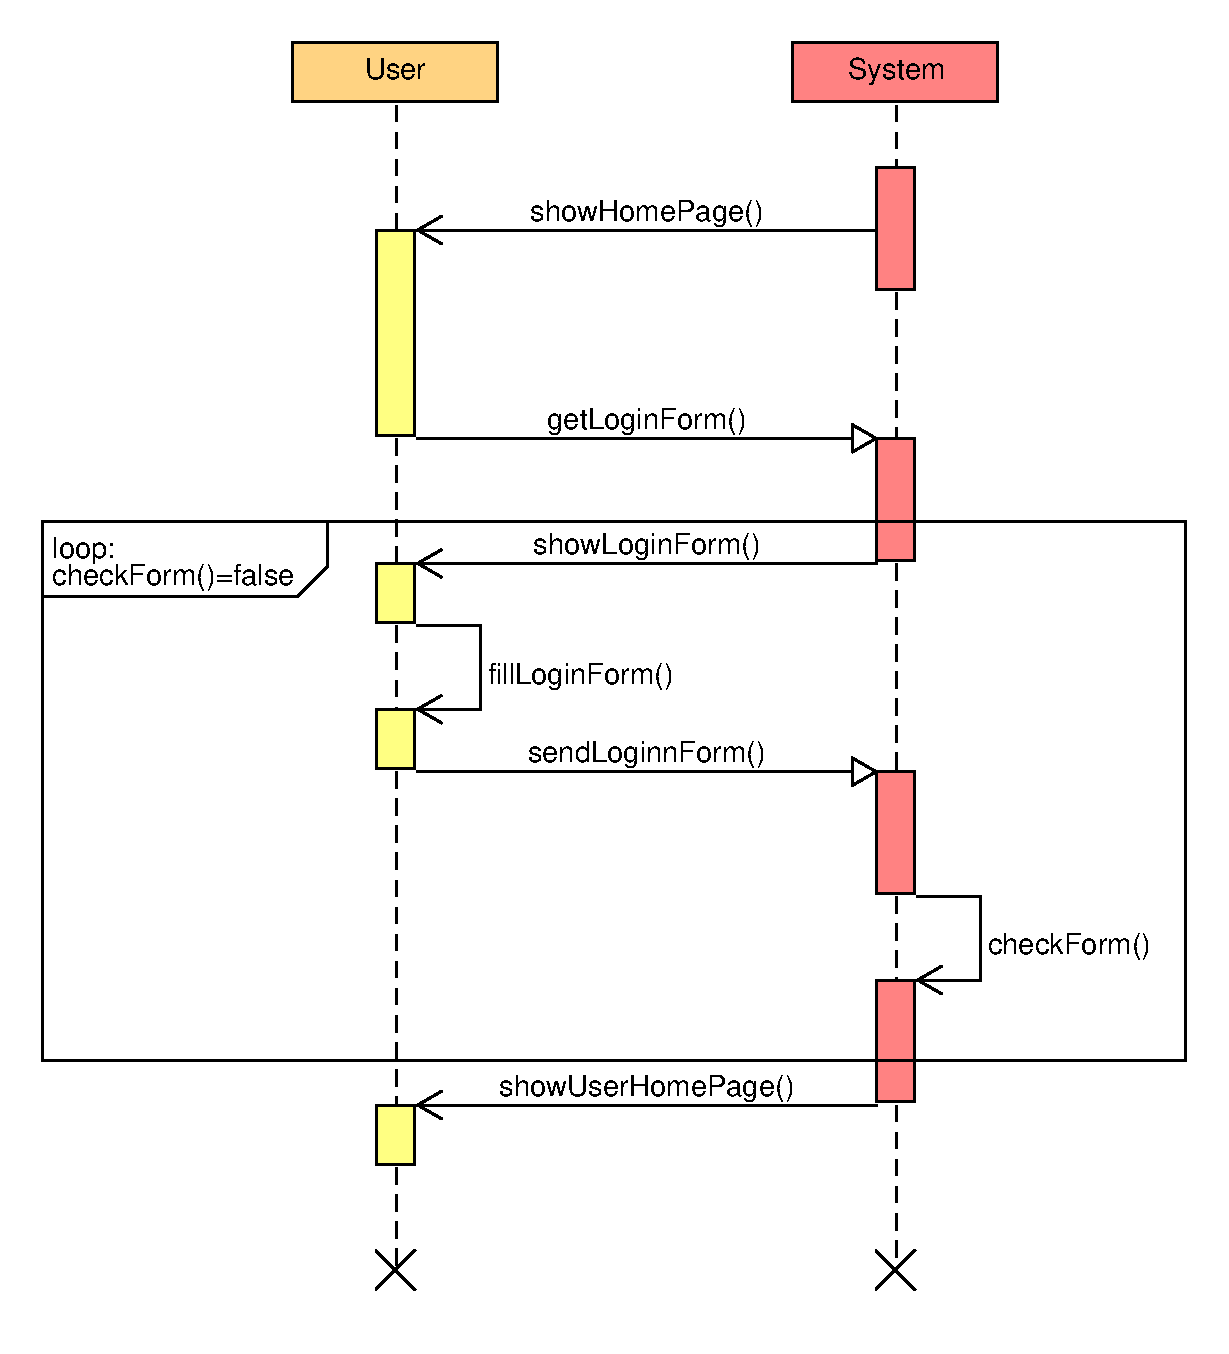
\includegraphics[width=\textwidth]{tex-images/sequence-login}
\caption{Log in sequence diagram}
\end{figure}


\begin{table}
\begin{center}
\begin{tabular}{lp{0.8\textwidth}}
\toprule
\textbf{Name}		&	\begin{itemize}
					\item Request for service
					\end{itemize}	\\
\textbf{Actors}		&	\begin{itemize}
					\item Passenger
					\item Taxi driver
					\end{itemize}	\\
\textbf{Entry conditions}	&	\begin{itemize}
					\item Passenger is logged into the system.
					\end{itemize}	\\
\textbf{Flow of events}	&	\begin{itemize}
					\item The passenger taps the \emph{Call a taxi now} button;
					\item The passenger inserts a destination address, the number of passengers, and if needed the starting address;
					\item The passenger confirms the request;
					\item The system receives the request;
					\item The system checks the taxi queue of the appropriate city zone and alerts the first taxi driver;
					\item The alerted taxi driver accepts the request and drives to the given address;
					\item The system informs the passenger that all went well and gives him the estimated time of arrival.	
					\end{itemize}	\\
\textbf{Exit conditions}	&	\begin{itemize}
					\item	A taxi driver accepts the request for service.
					\end{itemize}	\\
\textbf{Exceptions}	&	\begin{itemize}
					\item If the notified taxi driver declines, the system chooses the following in queue;
					\item If the request cannot be met for whatever reason, the system notifies the passenger.
					\end{itemize}	\\
\bottomrule
\end{tabular}
\caption{Request for service use case}
\end{center}
\end{table}

\begin{figure}
\centering
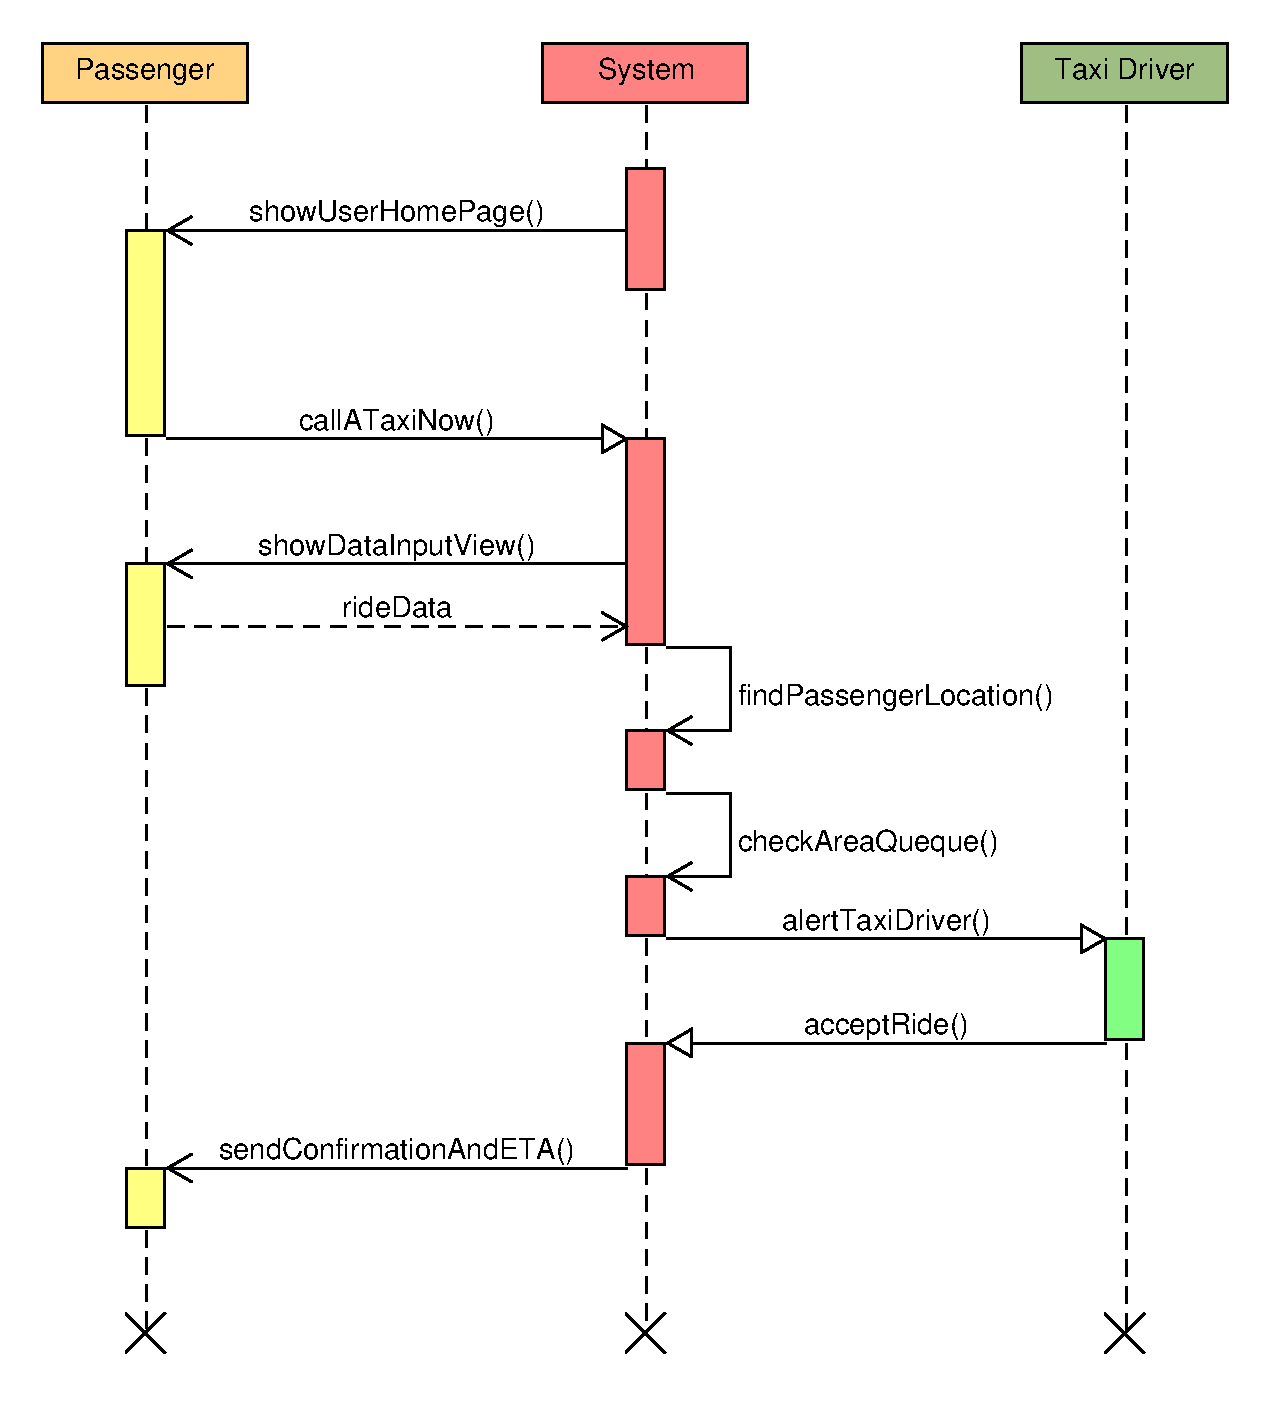
\includegraphics[width=\textwidth]{tex-images/sequence-rfs}
\caption{Request for service sequence diagram}
\end{figure}



\begin{table}
\begin{center}
\begin{tabular}{lp{0.8\textwidth}}
\toprule
\textbf{Name}		&	\begin{itemize}
					\item New reservation
					\end{itemize}	\\
\textbf{Actors}		&	\begin{itemize}
					\item Passenger
					\end{itemize}	\\
\textbf{Entry conditions}	&	\begin{itemize}
					\item	The passenger is logged in;
					\item	The system is showing user's home page.
					\end{itemize}	\\
\textbf{Flow of events}	&	\begin{itemize}
					\item	The passenger clicks on the \emph{New reservation} button;
					\item	The system shows him a form to be filled with all trip information (starting address, destination address, leaving date and time, number of passengers);
					\item	The user adds all information and clicks on the \emph{Confirm} button;
					\item	The system checks the information, analyses the request and confirms with a message;
					\item	The system generates a real time request ten minutes before the meeting time.
					\end{itemize}	\\
\textbf{Exit conditions}	&	\begin{itemize}
					\item	The reservation is correctly stored.
					\end{itemize}	\\
\textbf{Exceptions}	&	\begin{itemize}
					\item	If the information is wrong the system asks to rewrite it;
					\item	If the reservation can't be satisfied the system shows an error message.
					\end{itemize}	\\
\bottomrule
\end{tabular}
\caption{New reservation use case}
\end{center}	
\end{table}

\begin{figure}
\centering
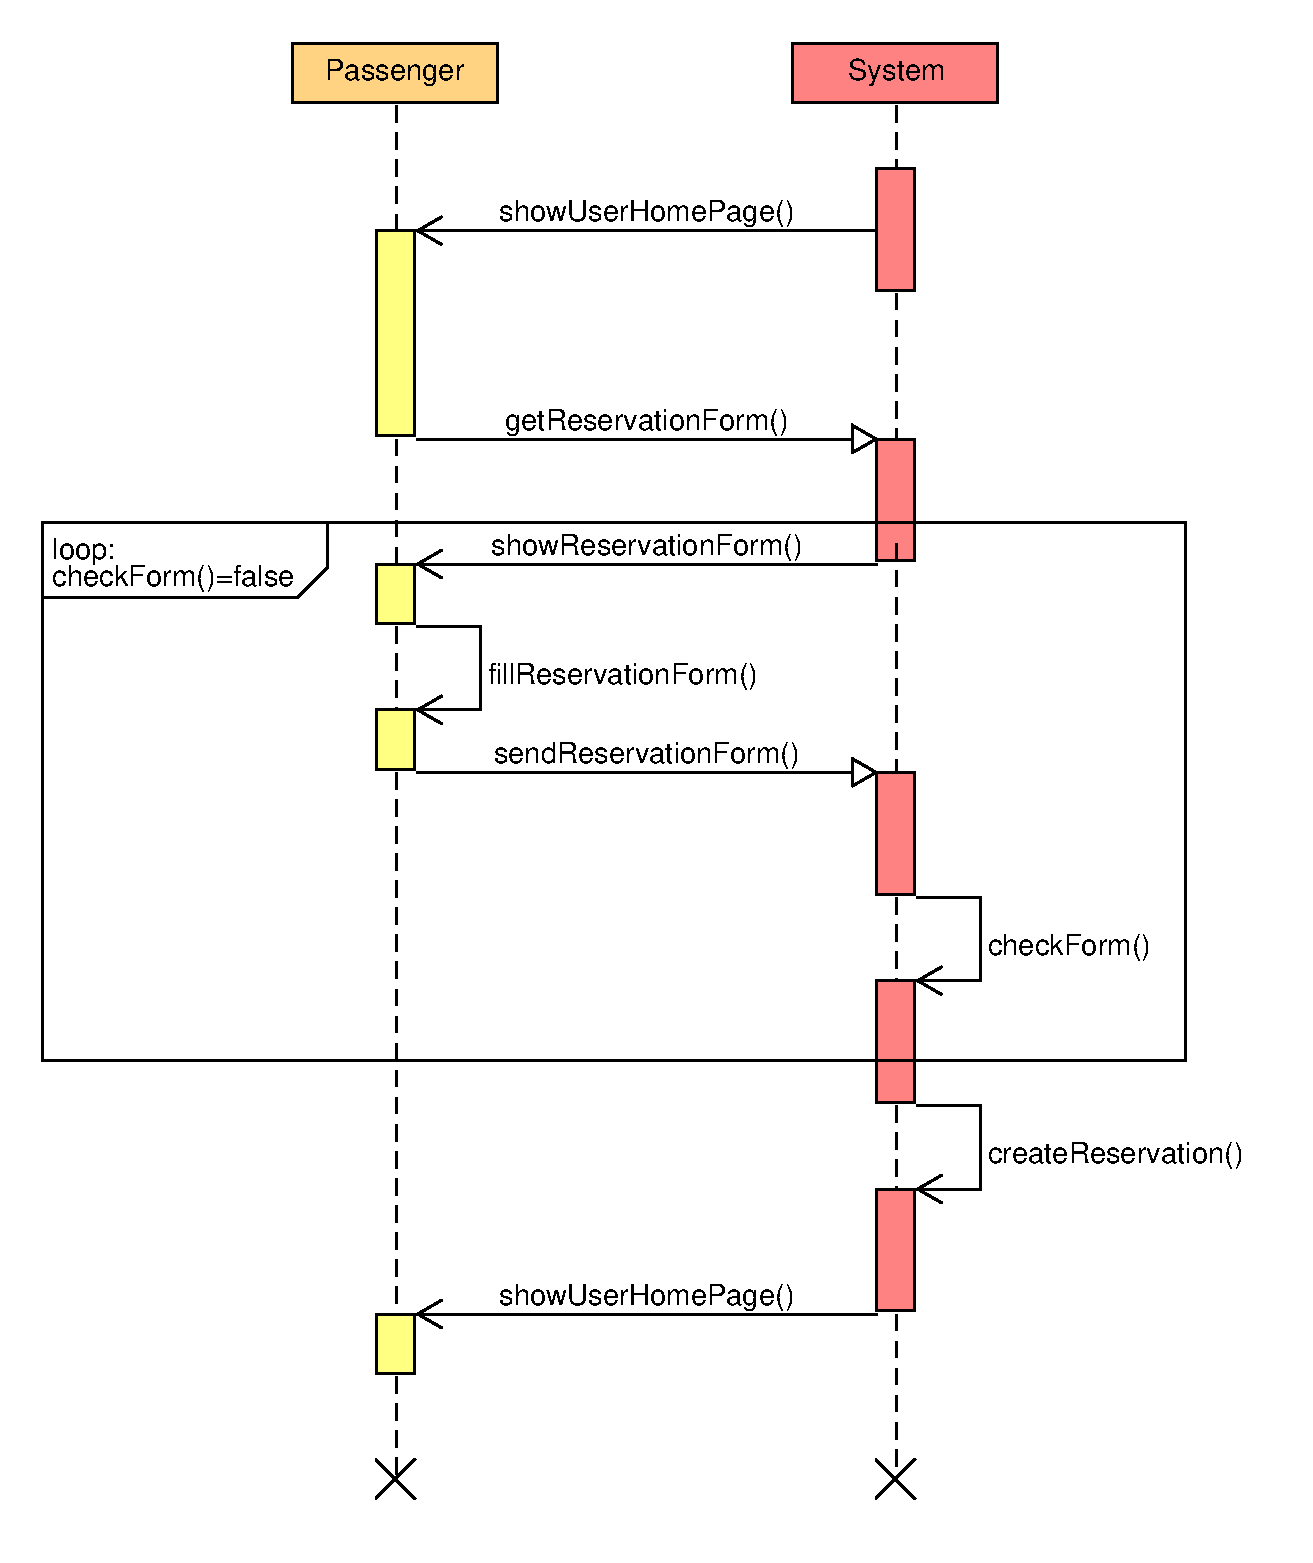
\includegraphics[width=\textwidth]{tex-images/sequence-new-reservation}
\caption{New reservation sequence diagram}
\end{figure}



\begin{table}				
\begin{center}
\begin{tabular}{lp{0.8\textwidth}}
\toprule
\textbf{Name}		&	\begin{itemize}
					\item Modify reservation
					\end{itemize}	\\
\textbf{Actors}		&	\begin{itemize}
					\item Passenger
					\end{itemize}	\\
\textbf{Entry conditions}	&	\begin{itemize}
					\item The passenger is logged in;
					\item	The system is showing user's home page.
					\end{itemize}	\\
\textbf{Flow of events}	&	\begin{itemize}
					\item	The passenger clicks on the \emph{Reservation history} button;
					\item	The system shows him all his reservations;
					\item	The user clicks on the reservation he wants to modify;
					\item	The system shows him a pop up window with two options: \emph{Modify} or \emph{Delete};
					\item	The user clicks on the \emph{Modify} button;
					\item	The system shows him a form to be filled with all trip information (starting address, destination address, leaving date and time, number of passengers);
					\item	The user adds all information and clicks on the \emph{Confirm} button;
					\item	The system checks the information, analyses the request and confirms with a message;
					\item	The system generates a real time request at the right moment to satisfy user reservation.
					\end{itemize}	\\
\textbf{Exit conditions}	&	\begin{itemize}
					\item	The reservation is correctly modified and stored.
					\end{itemize}	\\
\textbf{Exceptions}	&	\begin{itemize}
					\item	If there is no reservation in the history, the system shows an error message;
					\item	If it is too late to modify the reservation (less then two hours before the ride), the system shows an error message;
					\item	If the information is wrong the system asks to rewrite it;
					\item	If the reservation can't be satisfied the system shows an error message.
					\end{itemize}	\\
\bottomrule
\end{tabular}
\caption{Modify reservation use case}
\end{center}
\end{table}

\begin{figure}
\centering
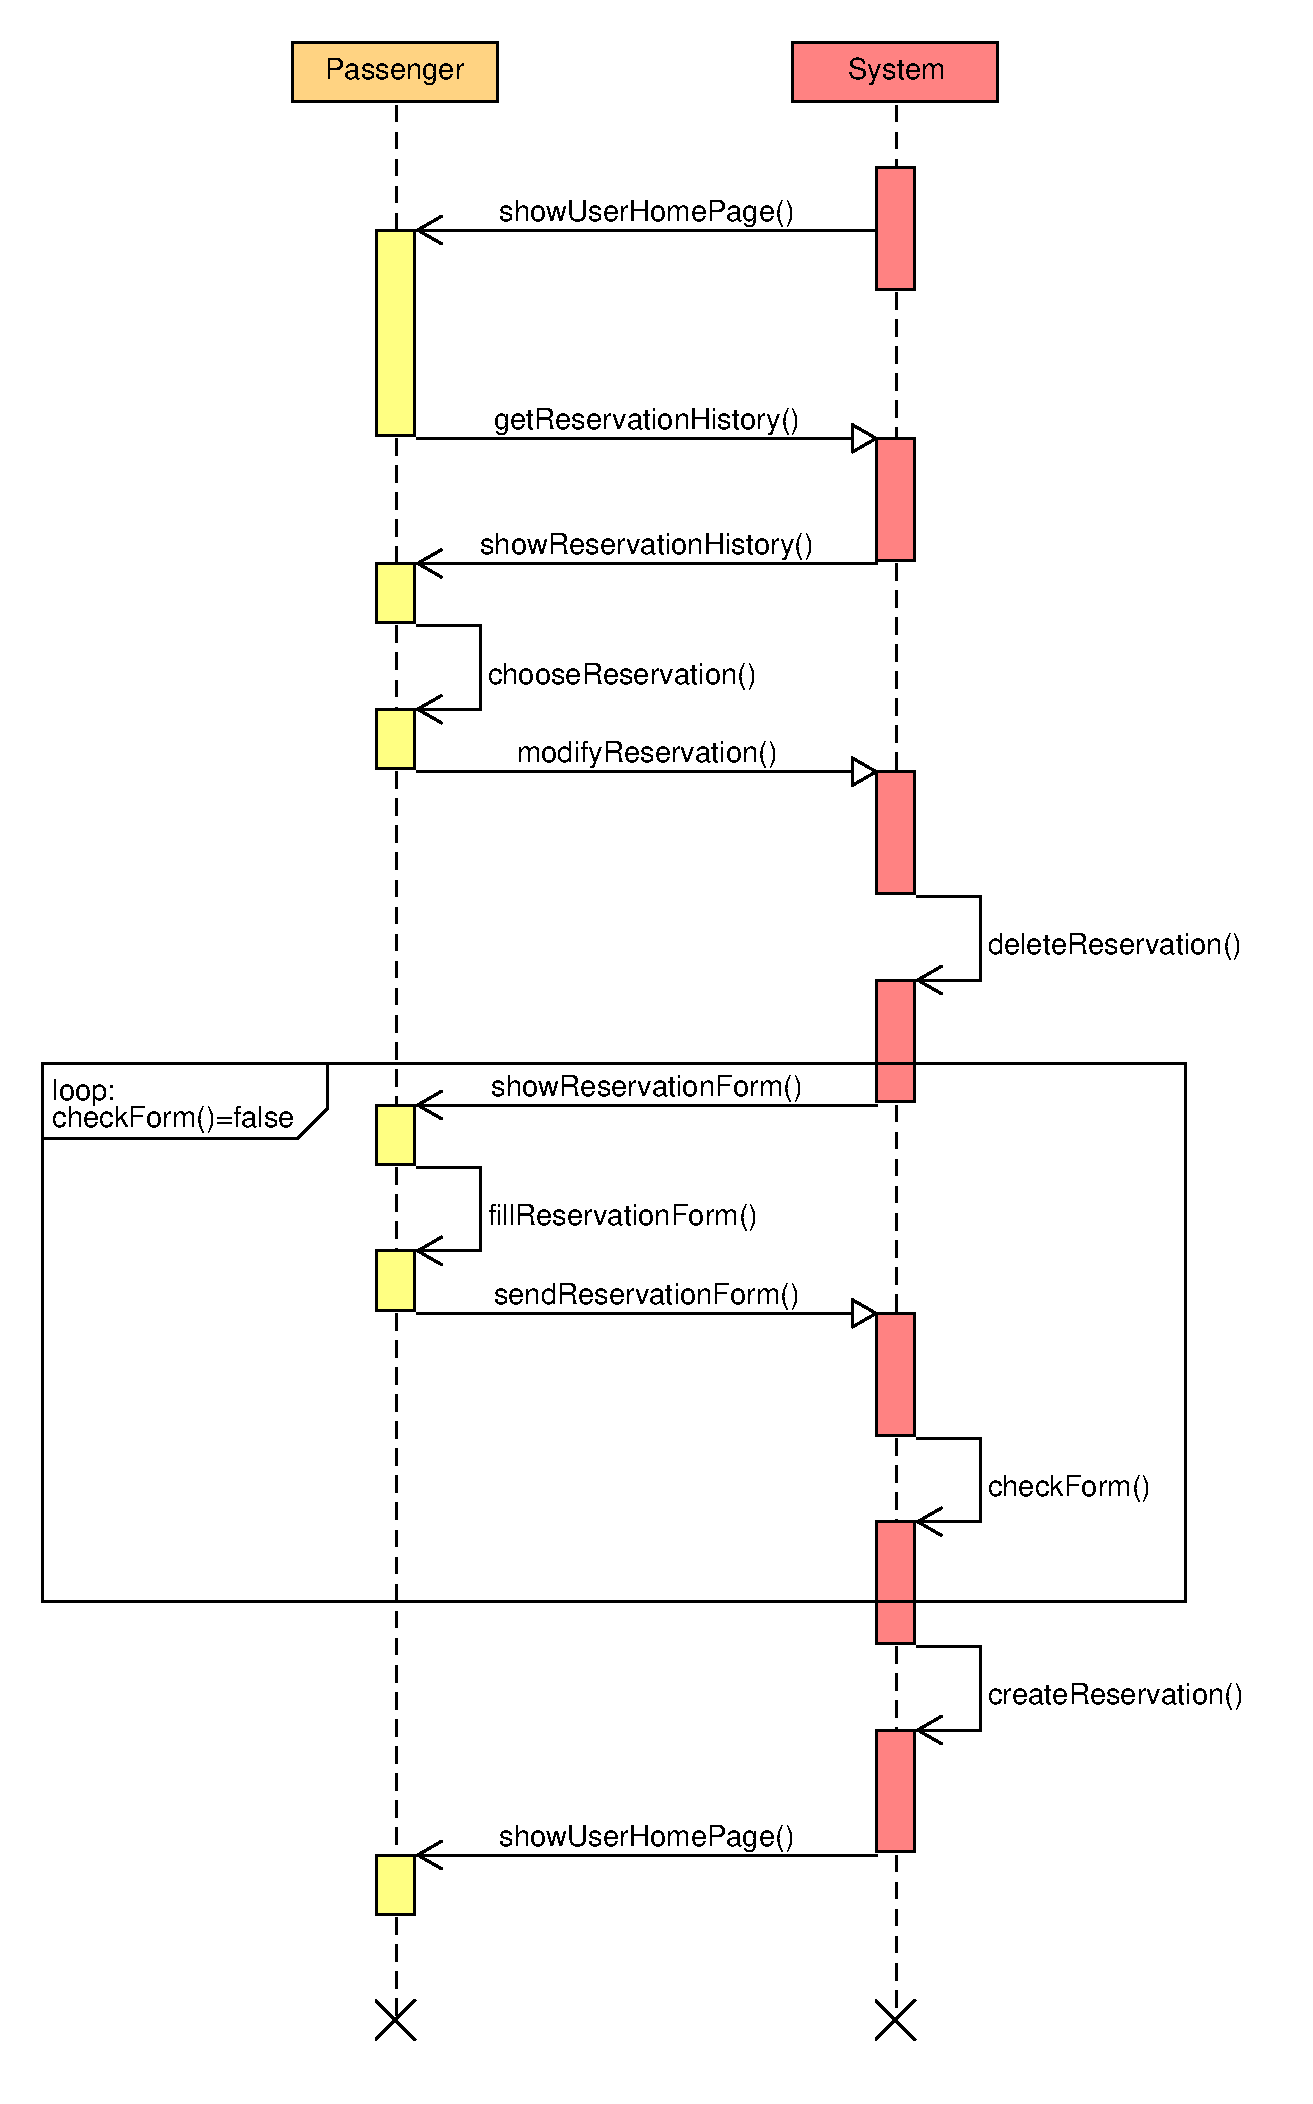
\includegraphics[width=\textwidth]{tex-images/sequence-modify-reservation}
\caption{Modify reservation sequence diagram}
\end{figure}



\begin{table}
\begin{center}
\begin{tabular}{lp{0.8\textwidth}}
\toprule
\textbf{Name}		&	\begin{itemize}
					\item Delete reservation
					\end{itemize}	\\
\textbf{Actors}		&	\begin{itemize}
					\item Passenger
					\end{itemize}	\\
\textbf{Entry conditions}	&	\begin{itemize}
					\item	The passenger is logged in;
					\item	The system is showing user's home page.
					\end{itemize}	\\
\textbf{Flow of events}	&	\begin{itemize}
					\item	The passenger clicks on the \emph{Reservation history} button;
					\item	The system shows him all his reservations;
					\item	The user clicks on the reservation he wants to delete;
					\item	The system shows him a pop up window with two options: \emph{Modify} or \emph{Delete};
					\item	The user clicks on the \emph{Delete} button;
					\item	The system deletes the reservation and shows reservation history.
					\end{itemize}	\\
\textbf{Exit conditions}	&	\begin{itemize}
					\item	The reservation is correctly deleted.
					\end{itemize}	\\
\textbf{Exceptions}	&	\begin{itemize}
					\item	If there is no reservation in the history, the system shows an error message.
					\end{itemize}	\\
\bottomrule
\end{tabular}
\caption{Delete reservation use case}
\end{center}
\end{table}

\begin{figure}
\centering
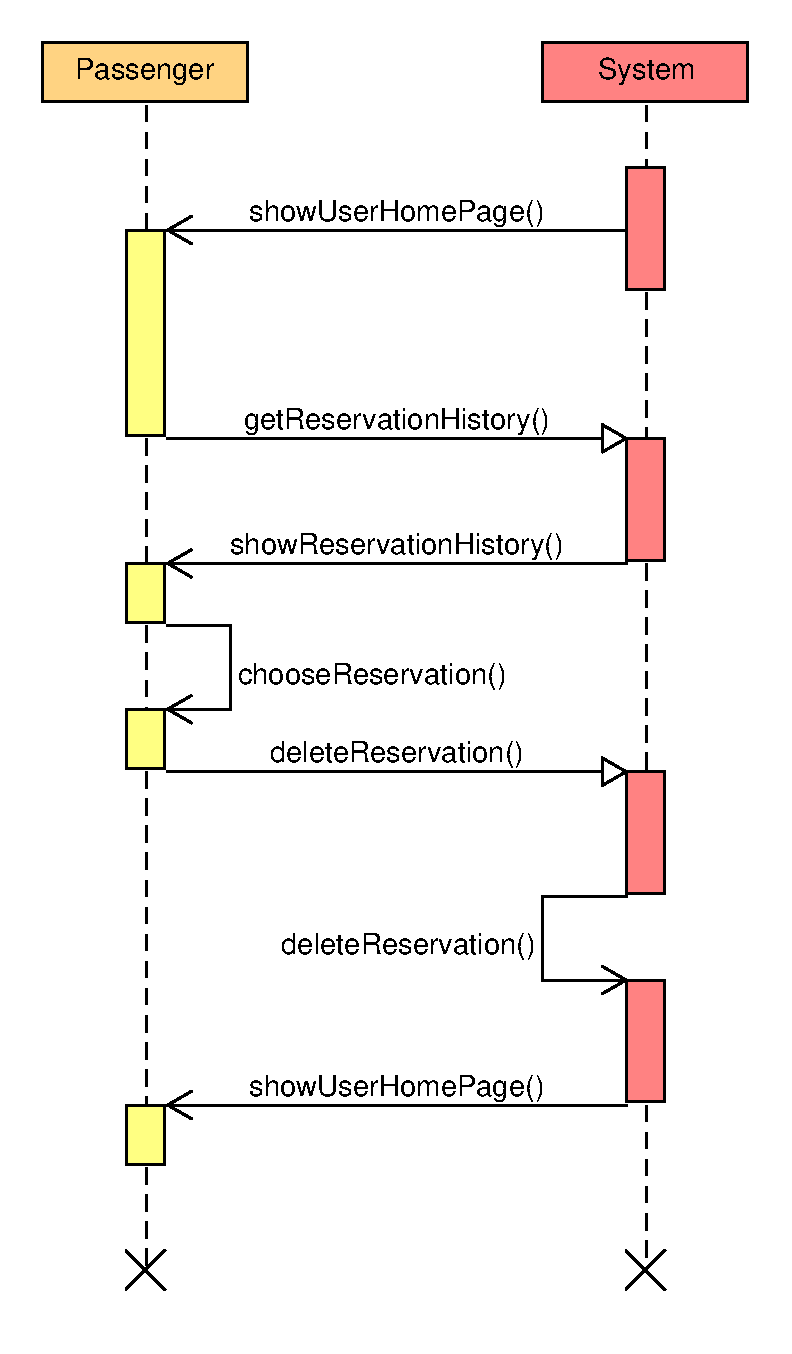
\includegraphics[width=\textwidth]{tex-images/sequence-delete-reservation}
\caption{Delete reservation sequence diagram}
\end{figure}




\begin{table}
\begin{center}
\begin{tabular}{lp{0.8\textwidth}}
\toprule
\textbf{Name}		&	\begin{itemize}
					\item Move taxi driver
					\end{itemize}	\\
\textbf{Actors}		&	\begin{itemize}
					\item Taxi driver
					\end{itemize}	\\
\textbf{Entry conditions}	&	\begin{itemize}
					\item Taxi driver is logged into the system and available.
					\end{itemize}	\\
\textbf{Flow of events}	&	\begin{itemize}
					\item The system checks the total coverage of taxis in the city and decides a taxi driver has to move;
					\item The system notifies the driver they have to move and where;
					\item The taxi driver confirms they are going to move.
					\end{itemize}	\\
\textbf{Exit conditions}	&	\begin{itemize}
					\item	The taxi driver reaches the designated zone.
					\end{itemize}	\\
\textbf{Exceptions}	&	\begin{itemize}
					\item The taxi driver does not move: the system either notifies them again or chooses another one.
					\end{itemize}	\\
\bottomrule
\end{tabular}
\caption{Move taxi driver use case}
\end{center}
\end{table}
\clearpage

\begin{figure}
\centering
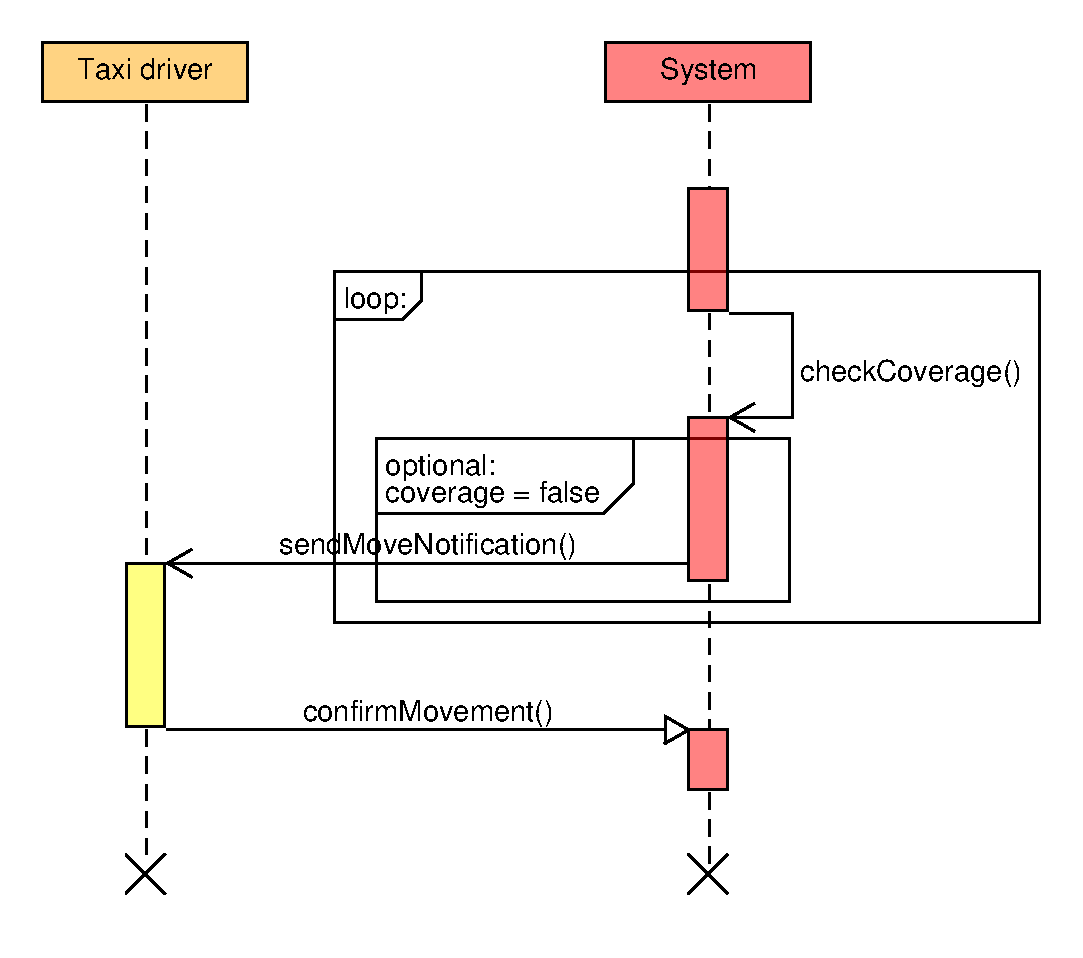
\includegraphics[width=\textwidth]{tex-images/sequence-move-taxi}
\caption{Move taxi driver sequence diagram}
\end{figure}




\begin{figure}
\centering
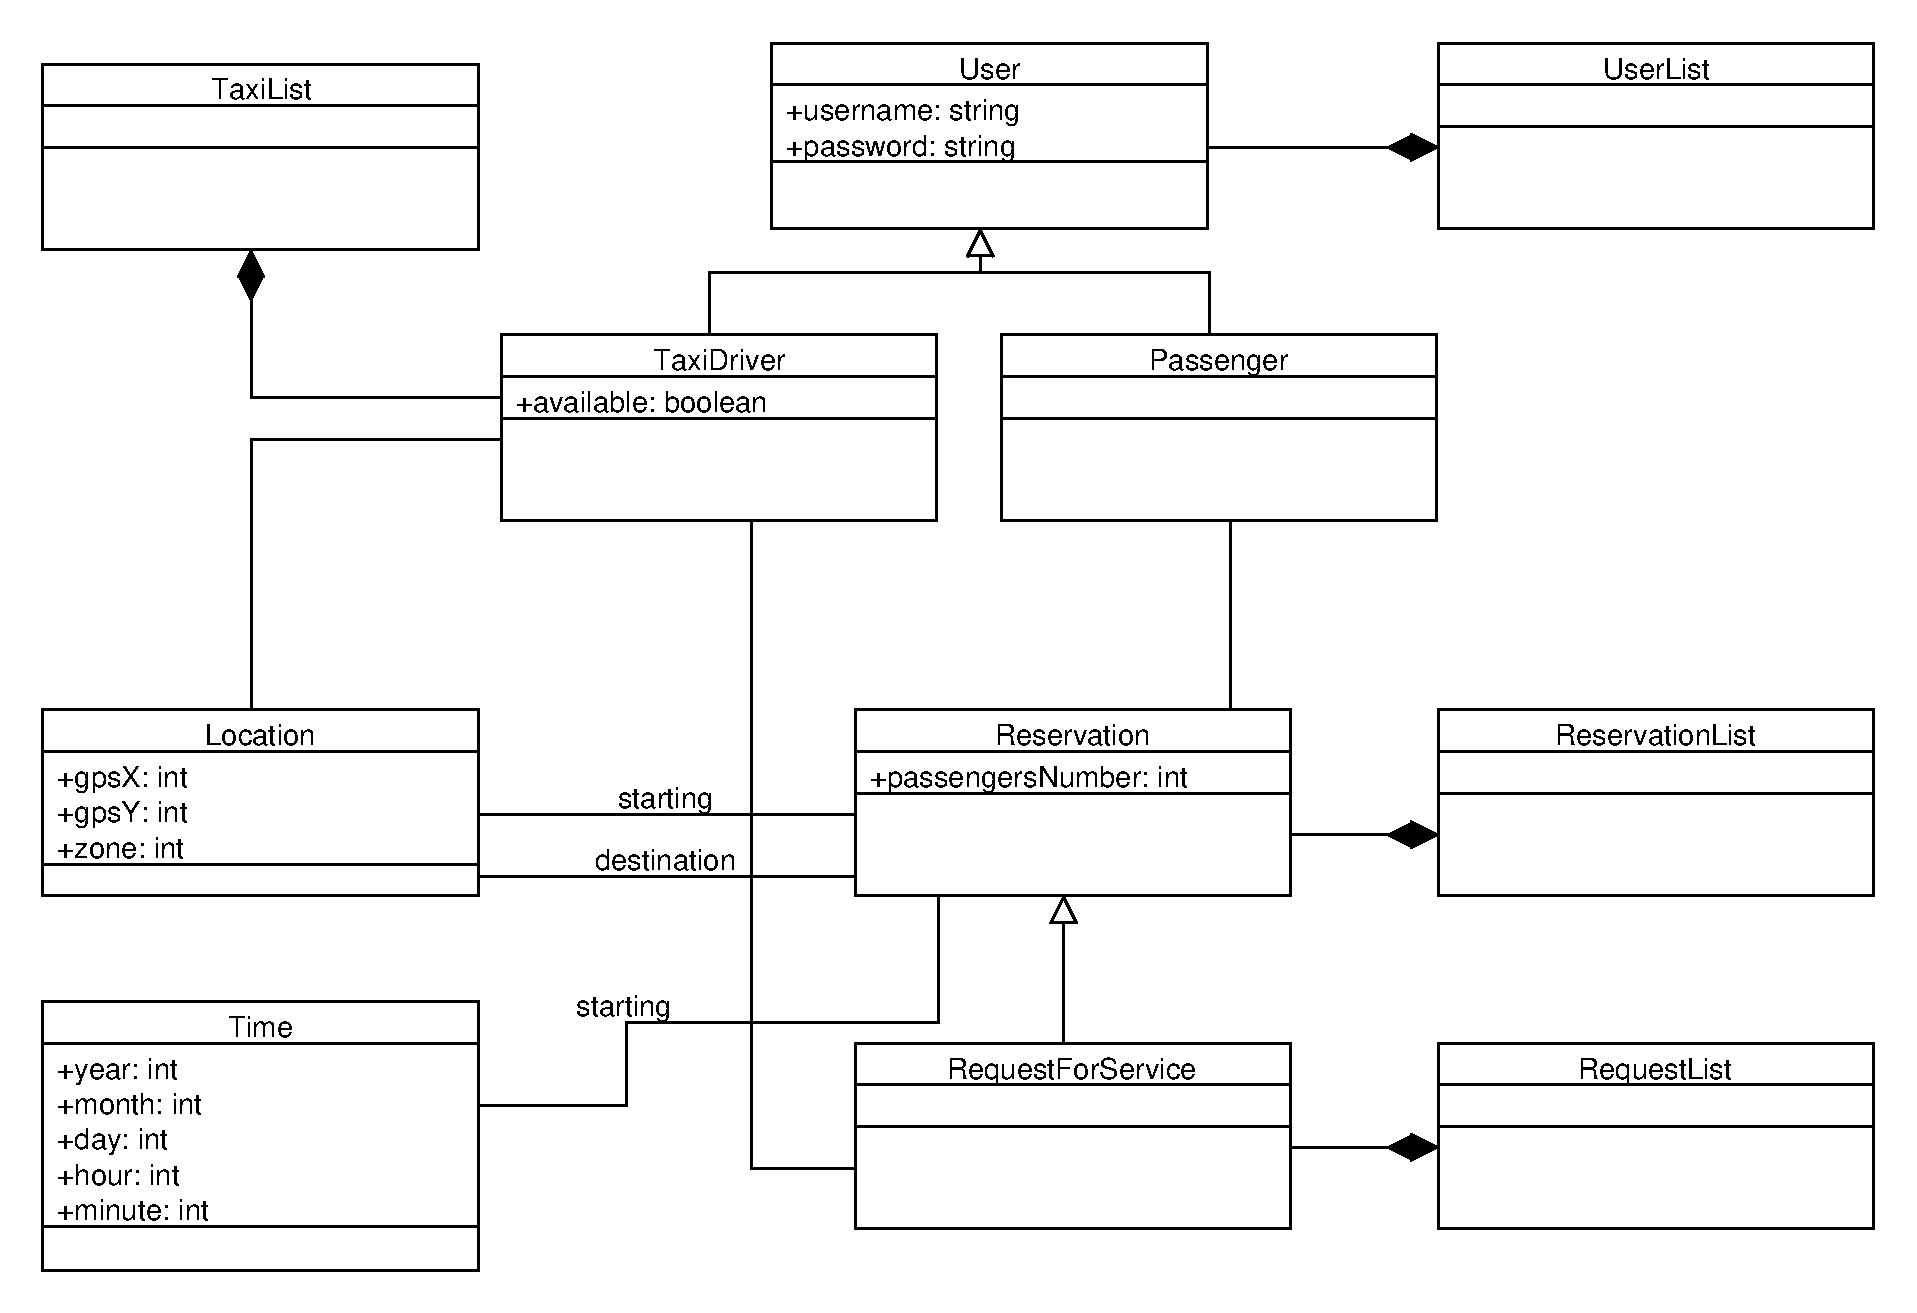
\includegraphics[width=\textwidth]{tex-images/class-diagram}
\caption{Main classes diagram}
\end{figure}

%%%%%%%%%%%%%%%%%%%%%%%%%%%%%%%%%%%%%%%%%
%%%%%%%%%%%%%%%%%%%%%%%%%%%%%%%%%%%%%%%%%

\section{Alloy model}
The following code is the Alloy modelization of the system that has been described in terms of requirements and goals in the previous sections. The \emph{Alloy Analyzer} tool was used to verify these properties, starting from the class diagram. The tool has proven the consistency of this model. In fact, no counterexample has been found and every predicate is consistent. A representation of the world extracted from this model is included.

\begin{figure}
\centering
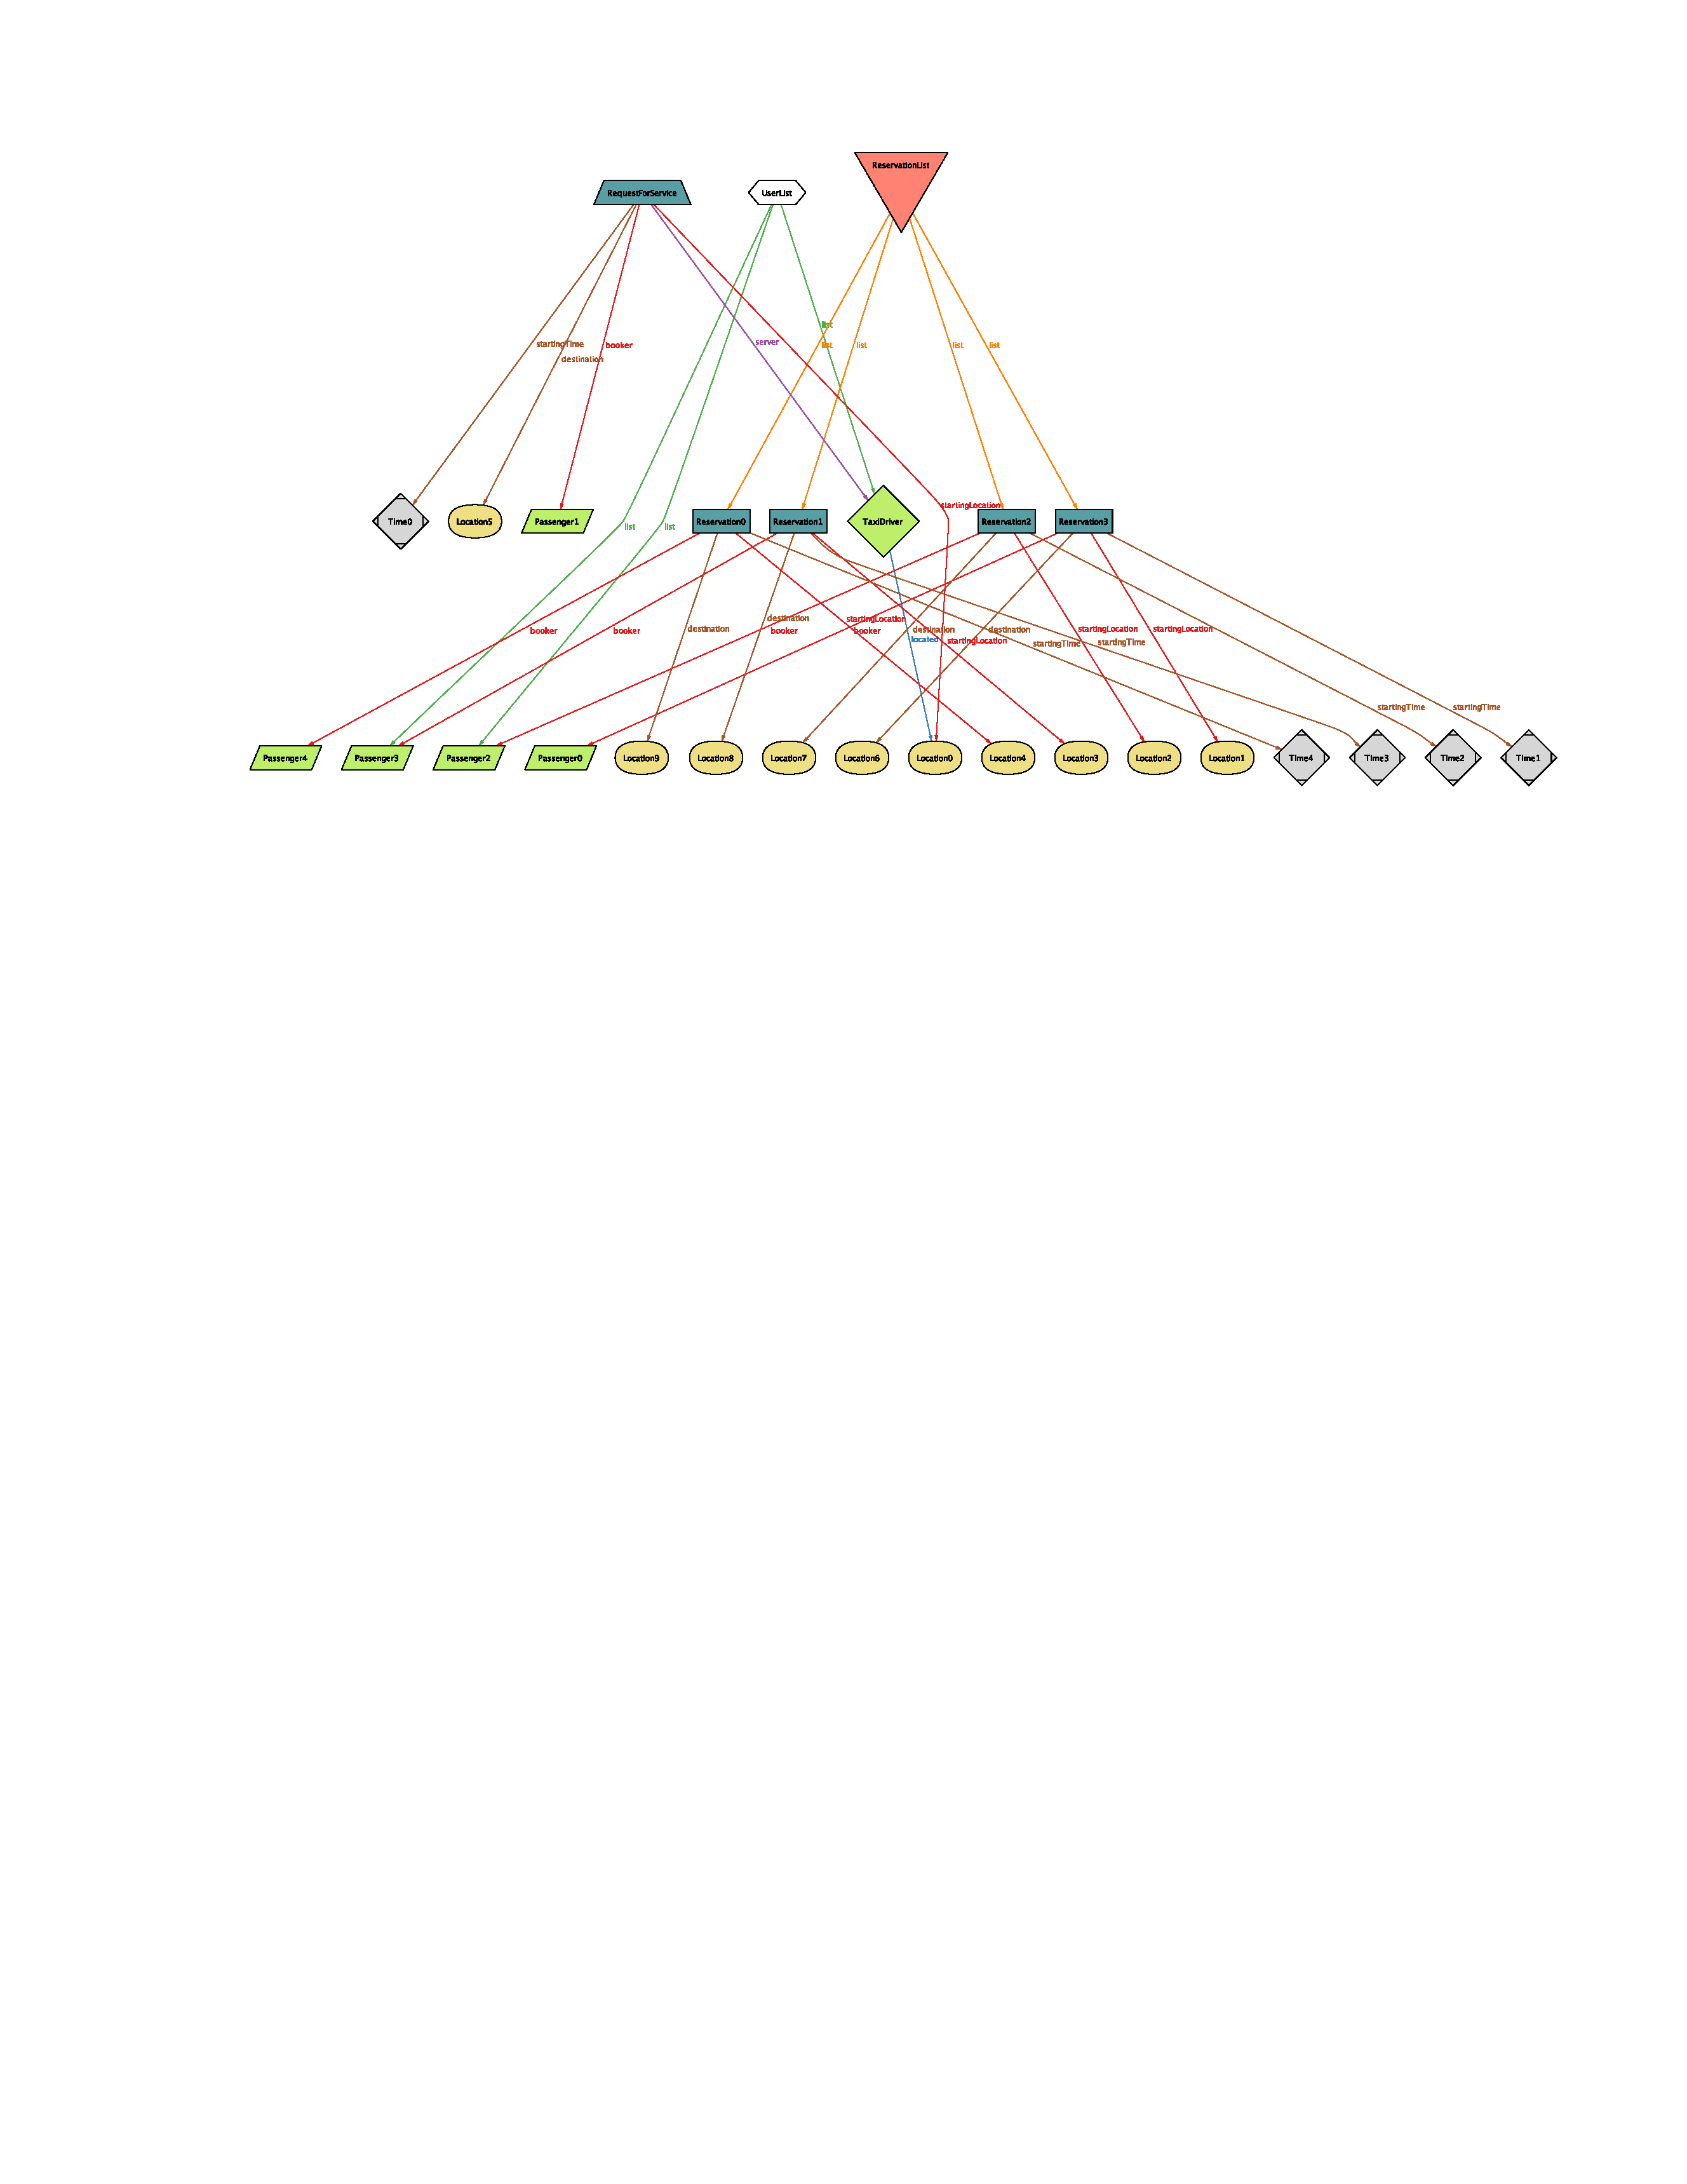
\includegraphics[width=\textheight, angle=90]{tex-images/alloy-world}
\caption{An alloy world representing this model}
\end{figure}

\alloyfile{alloy/Alloymodel.als}